% course:       CV
% teacher:      DongHui Wang
% author:       zju_cs / Yi Zhang / 21721190
% mail:         yizhangzc@gmail.com
% data:         2018/5
% environment:  ubuntu 16.04 / texlive-full / texlive-xetex      
% compiler:     xelatex / bibtex

\documentclass[a4paper]{article}

\usepackage{ctex}           % support chinese
\usepackage{geometry}       % setting margin
\usepackage{setspace}       % setting space
\usepackage{algorithm}      % 
\usepackage{caption}        % support caption
\usepackage{amsmath}        % support newtheorem
\usepackage{graphicx}       % support insert iamge


\title{三元组损失在重识别领域的应用}
\date{2018-05}
\author{张毅\hspace{1em}21721190}

\geometry{left=3cm,right=3cm,top=3cm,bottom=3cm}
\setcounter{tocdepth}{3}
\doublespacing

\begin{document}
    
    %%%%%%    标题   %%%%%%%%%%%%%%
    \pagenumbering{gobble}
    \begin{center}
        \doublespacing
        
        \Large \textbf{三元组损失在重识别领域的应用}

        \normalsize 姓名:张毅 \qquad 学号:21721190 \qquad 邮箱: yizhangzc@gmail.com \qquad 日期:2018-5
    \end{center}
    

    %%%%%%    报告简述   %%%%%%%%%%%%%%
    \pagenumbering{arabic}
    \section{报告简述}

    本次报告选题为三元组损失(tirplet loss)在重识别(Re-Identification)领域的应用,题目的选择是由于前段时间恰巧对triplet loss进行了简单的了解,本次报告在之前的基础上对三元组损失相关内容做一个梳理与总结。报告中涉及到的文章包括CVPR 2015-2017, ICCV2017等会议文章。当前CVPR2018只公布了接收文章编号,而在接受作者自己放出的论文中暂时没有发现相关的内容,所以报告中没能对CVPR2018的论文进行跟踪。

    本次报告以及课后作业\&技术报告均已上传至github仓库(yizhangzc/course),报告包含tex代码以及pdf文件,代码由python语言实现。

    %%%%%%    三元组损失    %%%%%%%%%%%%%%
    \section{三元组损失}

    三元组损失在2015年首次被Google用于人脸识别系统FaceNet\cite{cvpr15facenet},本章将基于该论文介绍三元组损失。FaceNet直接学习人脸图像到欧几里得空间的映射,空间距离表示人脸图像的相似性。当学习好这个映射后,人脸识别、验证等任务可以很容易地在这个空间完成。

    在此之前,基于深度模型的人脸识别大多基于分类模型进行训练,然后将网络中间层作为人脸图像的特征表示用于人脸识别任务中。这类方法对于训练集之外的用户不能很好的适配,并且通常中间层的图像特征表示维度很高,它的问题是不直接且效率低。

    在论文中,FaceNet使用三元组损失作为损失函数,模型输出即是仅128维的embedding。三元组包含一个称为锚的样本$x_i^a$,与锚相匹配的正样本$x_i^p$和与锚不匹配的负样本$x_i^n$。三元组损失函数鼓励锚与负样本之间的距离比锚与正样本之间的距离大于某个预定义的阈值。FaceNet网络模型如图1所示。

    \begin{figure}[H]
        \centering
        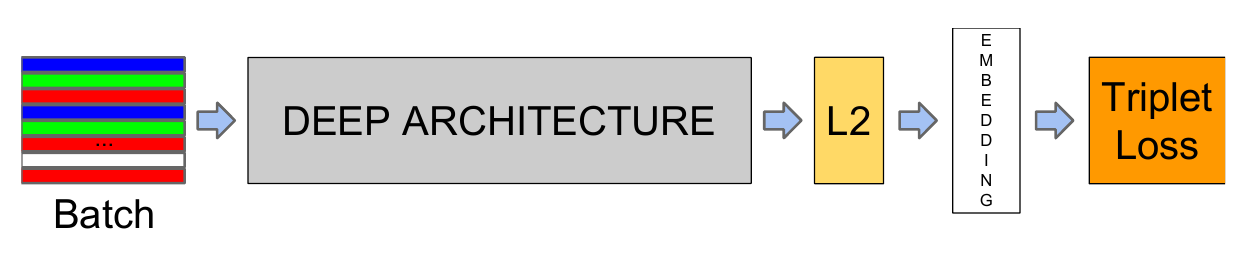
\includegraphics[width=0.9\linewidth]{./images/facenet_structure.png}
        \caption{FaceNet网络结构}
        \label{fig:facenet_structure}
    \end{figure}
    
    其中,FaceNet使用了深度卷积网络端对端的学习人脸图像的embedding。其直接使用反应人脸识别目标的三元组损失。即,学习从图像$x$到embedding空间$R^d$的映射$f(x)$,使得来自相同身份的所有embedding之间的距离小,而一对来自不同身份的embedding之间的距离大,见图2。作者认为三重损失更适合于人脸识别。

    \begin{figure}[H]
        \centering
        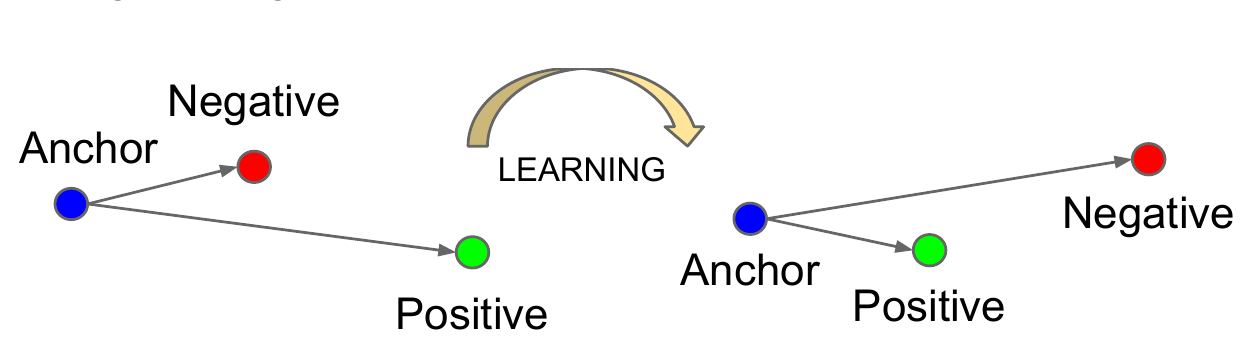
\includegraphics[width=0.9\linewidth]{./images/Triplet_loss_demo.png}
        \caption{三元组损失}
        \label{fig:triplet_loss_demo}
    \end{figure}

    对于一特定个体的人脸图像$x_i^a$,来自相同个体的其他人脸图像$x_i^p$,来自不同个体的人脸图像$x_i^n$。我们希望$x_i^a$与$x_i^p$的距离小于$x_i^a$和$x_i^n$的距离。可以由公式(1)表示:

    \begin{equation}
        ||x_i^a-x_i^p||_2^2 + \alpha < ||x_i^a-x_i^n||_2^2, \forall (x_i^a,x_i^p,x_i^n) \in \tau
    \end{equation}
    其中,$\alpha$表示预定义的阈值。若embedding由$f(x)R^d$表示,它将图像映射到d维欧几里得空间中。损失函数可由公式(2)表示:

    \begin{equation}
        \sum_i^N \big[ ||f(x_i^a)-f(x_i^p)||_2^2 - ||f(x_i^a) - f(x_i^n)||_2^2 + \alpha \big]_+
    \end{equation}
    其中$[x]_+=max[0,x]$。

    挑选不满足三元组约束的个体训练模型对加快收敛至关重要。理想情况下,对于$x_i^a$,我们希望选择同一个体的不同图片$x_i^p$,使$argmax_{x_i^p}||f(x_i^a)-f(x_i^p)||_2^2$,同样的,选择$x_i^n$,使$argmin_{x_i^n}||f(x_i^a)-f(x_i^n)||_2^2$。实际情况下,在整个数据集上计算$argmax$与$argmin$不可行。而且可能使错误标记的样本影响到模型的训练。文中提出两种可选的三元组挑选方式:(1)离线选择三元组,在固定的训练间隔使用当前网络在某个样本子集上计算$argmax$与$argmin$。(2)在线选择三元组,在每个batch计算$argmax$与$argmin$。

    文中使用了两种深度卷积网络(Zeiler\&Fergus style networks和Inception)进行实验,采用了约八百万个体的将近1亿2亿到张人脸缩略图训练模型。最后,在四类数据集(hold-out测试集、个人照片、LFW数据集、Youtube Faces DB)上评价FaceNet,并对一些超参对模型的影响进行了简单的分析。
    
    超参对模型影响:(1)随着神经网络深度增加,计算量增加,准确率也增加;(2)模型对图像质量不敏感;(3)128维的embedding在是实验中最为合适;(4)随着训练数据量的增加,准确率也随之增加。

    FaceNet在LFW数据集上取得了99.63\%$\pm$0.09的准确率;在Youtube Faces DB数据集上获得了95.12\%$\pm$0.39的结果。

    
    %%%%%%    改进的三元组损失    %%%%%%%%%%%%%%
    \section{改进的三元组损失}

    三元组损失在重识别领域获得了很好的效果,之后,基于三元组损失,许多改进版本被相继提出,本章对一些比较有名的三元组损失的改进版进行简要介绍。

    \subsection{Coupled Clusters Loss}

    Liu等人认为在处理随机选择的三元组时,存在一些特殊情况,三元组损失可能被错误地判断。给定3个样本(锚,与锚匹配的正样本,与锚不匹配的负样本),有两种不同的方式构建三元组作为网络的输入数据。图3中,在左边的情况下,由于类内距离大于类间距离,所以三重态丢失可以容易地检测到异常距离关系。右边情况有则不同。 由于锚与正样本之间的距离确实小于锚点与负样本之间的距离,所以三元组损失为0。因此,网络将在反向传播期间忽略这个三元组。

    \begin{figure}[H]
        \centering
        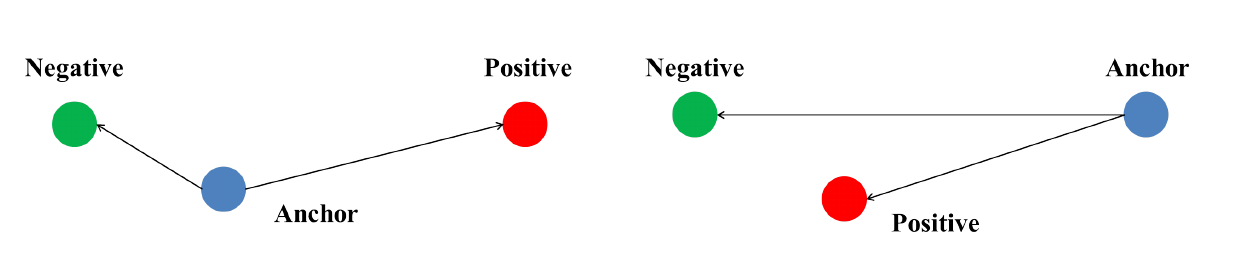
\includegraphics[width=0.9\linewidth]{./images/cvpr16_error_case.png}
        \caption{三元组}
        \label{fig:cvpr16_error_case}
    \end{figure}

    鉴于上面的情况,Liu等人提出Coupled Clusters Loss\cite{cvpr16triplet},其中,三元组被两个图像集取代:一个正集和一个负集。正集$X^p = \{x_1^p,\cdots,x_{N_p}^p\}$包含相同个体的$N_p$个图像,负集$X^n = \{x_1^n,\cdots,x_{N_n}^n\}$包含其它不同个体的$N_n$个图像。 假设同一个体的样本应该位于$d$维欧几里得空间中的共同中心点附近。则正集中的样本应该形成一个集群,而负集中的样本应该保持相对较远。基于此,Coupled Clusters Loss由公式(3)表示。

    \begin{equation}
        \sum_i^{N^p} \frac{1}{2} max \big \{0,||f(x_i^p)-c^p||_2^2 + \alpha - ||f(x_*^n) - c^p||_2^2 \big\}
    \end{equation}
    其中,$c^p$表示正样本的中心,$x_*^n$表示离正样本中心最近的负样本。相比原始的三元组损失,(1)距离度量的是样本与一个中心的距离,而非与随机选择的锚样本;(2)损失函数定义在多个样本上,而不只是三元组。

    \subsection{Beyond triplet loss}

    Chen等人认为传统的三元组损失可能在测试集上泛化效果一般,主要是因为类内方差依然比较大。文章提出来一种四元组损失\cite{cvpr17beyond},在传统三元组损失的基础上增加了新的约束,用于减小类内方差,增加类间方差。

    \begin{equation}
        \sum_{i,j,k}^N \big [g(x_i,x_j)^2 - g(x_i,x_k)^2 + \alpha_1 \big]_+ + \sum_{i,j,k,l}^N \big [g(x_i,x_j)^2 - g(x_l,x_k)^2 + \alpha_2 \big]_+
    \end{equation}
    其中,$s_i=s_j,s_l \neq s_k,s_i \neq s_l, s_i \neq s_k$,$g(x_1,x_2)$表示$x_1$与$x_2$之间的相似度。损失函数包含两项,前一项是传统的三元组损失,后一项用于进一步缩小类内差距。由于前一项更加重要,因此作者控制$\alpha_1>\alpha_2$。

    
    \subsection{Improved triplet loss function}

    Liao等人基于三元组损失对其进行了修改,提出了Improved triplet loss function\cite{iccv17triplet},见公式(5)。

    \begin{equation}
        max \big \{ 0, \lambda || F_i^0 - F_i^+ ||_2^2 - \beta || F_i^0 - F_i^- ||_2^2 + \alpha \big \}
    \end{equation}

    原始的三元组损失要求两个相同个体样本之间的距离比两个不同个体样本之间的距离更近。作者提出了更加普遍的表示方式,通过两个参数分别控制两个距离项。如图4所示。


    \begin{figure}[H]
        \centering
        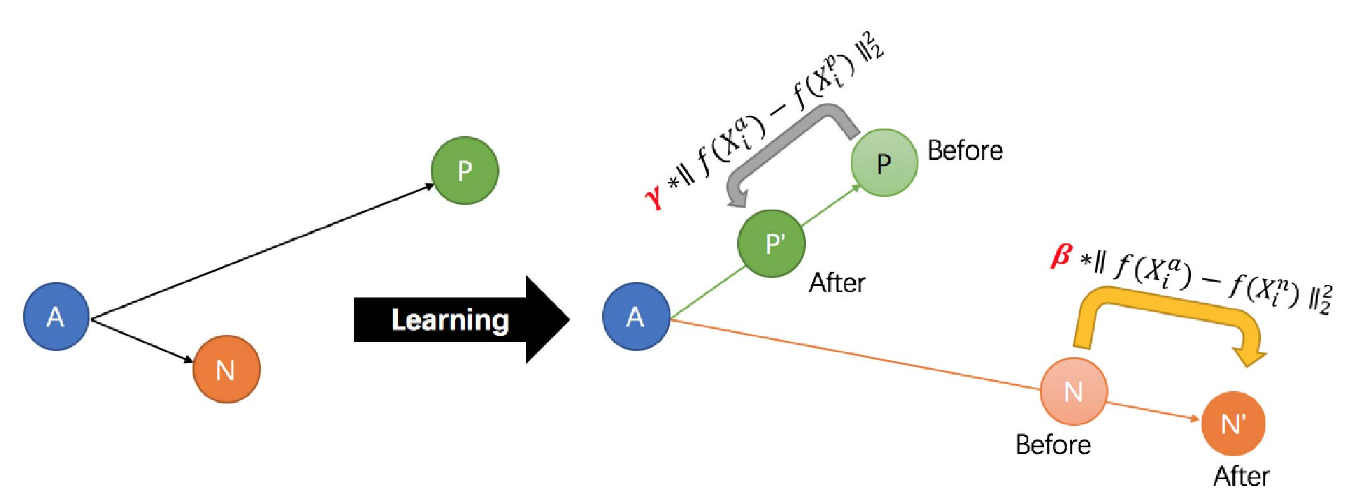
\includegraphics[width=0.7\linewidth]{./images/iccv17_tri.png}
        \caption{Improved triplet loss function}
        \label{fig:cvpr16_error_case}
    \end{figure}

    \section{总结}

    1)传统的分类通常是大类别的识别,但是有些需求是要精确到更细粒度的识别,比如人脸识别。三元组损失最主要应用就是细粒度的识别,如face identification,person re-identification,vehicle re-identification的各种identification识别问题。当类别非常大时,传统的基于softmax的分类网络输出层参数会非常多,且分类效果下降。但是三元组损失学习距离,参数少,且能有效的进行距离的度量。2)三元组的选择对基于三元组损失的模型非常重要。3)对于人脸识别等应用,基于分类的模型容易对新个体的泛化能力弱,三元组损失通过直接学习距离能有效避免。4)当前对三元组损失的改进版本有许多,需要针对不同的任务以及数据特定进行选择。

    %%%%%%    索引    %%%%%%%%%%%%%%
    \bibliography{final_report}
    \bibliographystyle{ieeetr}

\end{document}